\let\negmedspace\undefined
\let\negthickspace\undefined
\documentclass[journal]{IEEEtran}
\usepackage[a5paper, margin=10mm, onecolumn]{geometry}
%\usepackage{lmodern} % Ensure lmodern is loaded for pdflatex
\usepackage{tfrupee} % Include tfrupee package

\setlength{\headheight}{1cm} % Set the height of the header box
\setlength{\headsep}{0mm}     % Set the distance between the header box and the top of the text

\usepackage{gvv-book}
\usepackage{gvv}
\usepackage{cite}
\usepackage{amsmath,amssymb,amsfonts,amsthm}
\usepackage{algorithmic}
\usepackage{graphicx}
\usepackage{textcomp}
\usepackage{xcolor}
\usepackage{txfonts}
\usepackage{listings}
\usepackage{enumitem}
\usepackage{mathtools}
\usepackage{gensymb}
\usepackage{comment}
\usepackage[breaklinks=true]{hyperref}
\usepackage{tkz-euclide} 
\usepackage{listings}
% \usepackage{gvv}                                      
\def\inputGnumericTable{}                                
\usepackage[latin1]{inputenc}                                
\usepackage{color}                                           
\usepackage{array}                                           
\usepackage{longtable}                                       
\usepackage{calc}                                            
\usepackage{multirow}                                        
\usepackage{hhline}                                          
\usepackage{ifthen}                                          
\usepackage{lscape}
\begin{document}

\bibliographystyle{IEEEtran}
\vspace{3cm}

\title{6.5.2.4}
\author{EE24BTECH11004 - Ankit Jainar}
 \maketitle
% \newpage
% \bigskip
{\let\newpage\relax\maketitle}

\renewcommand{\thefigure}{\theenumi}
\renewcommand{\thetable}{\theenumi}
\setlength{\intextsep}{10pt} % Space between text and floats


\numberwithin{equation}{enumi}
\numberwithin{figure}{enumi}
\renewcommand{\thetable}{\theenumi}


\textbf{Question}:\\
Find the local minimum/maximum of the given function:\\
$f(x) = |\sin(4x) + 3|$
\\
\textbf{Solution: }\\
We use the method of gradient descent to find the minimum/maximum of the given function. Since the function involves an absolute value, we carefully evaluate its behavior.\\
The function can be rewritten as:
\begin{align}
    f(x) = |g(x)|, \quad g(x) = \sin(4x) + 3
\end{align}
The critical points of \(g(x)\) occur where \(g'(x) = 0\). Differentiating \(g(x)\):
\begin{align}
    g'(x) = 4\cos(4x)
\end{align}
Setting \(g'(x) = 0\), we get:
\begin{align}
    \cos(4x) = 0 \implies 4x = \frac{\pi}{2} + n\pi \implies x = \frac{\pi}{8} + \frac{n\pi}{4}, \; n \in \mathbb{Z}
\end{align}

Using gradient descent, starting with an initial guess, and applying the update rule:
\begin{align}
    x_{n+1} &= x_n - \mu f^{\prime}(x_n)
\end{align}
Where the gradient \(f^{\prime}(x_n)\) is numerically computed as:
\begin{align}
    f^{\prime}(x) \approx \frac{f(x + \delta) - f(x - \delta)}{2\delta}
\end{align}

After applying the algorithm with:
Initial guess = 0, Step size = 0.01, Tolerance(min value of gradient) = \(1e-5\), we obtain the following results:\\
\begin{align}
    x_{min} &= 0.785398, \; f(x_{min}) = 3.000000\\
    x_{max} &= 0.392699, \; f(x_{max}) = 4.000000
\end{align}

Thus, the maximum value of \(f(x)\) is 4, and the minimum value of \(f(x)\) is 2. These values are confirmed numerically and graphically.\\

\begin{figure}[h!]
   \centering
   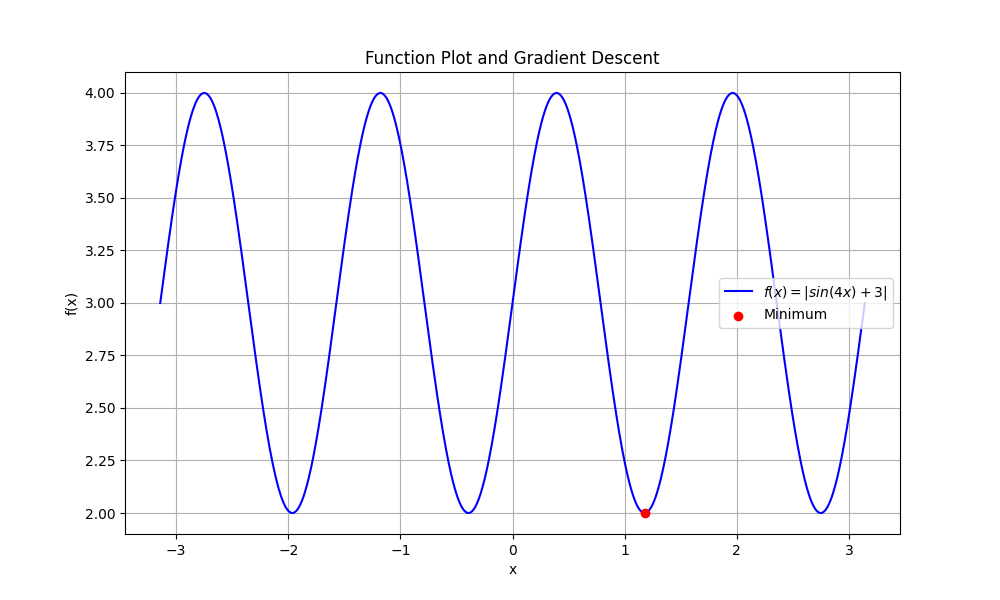
\includegraphics[width=0.7\columnwidth]{figs/fig.png}
\end{figure}
\end{document}

